\subsection{Услов}

У програмирању се често постављају "да" или "не" питања и доносе се одлуке шта урадити у односу на одговор. На пример, може се поставити питање: "Да ли студирате математику мање од 8 година?" и ако је одговор "Да", то се може протумачити као: "Ви сте сјајан студент!".

Често се комбинују услови(питања) и одговори у оквиру \emph{if}\index{Python!if@\emph{if}} наредбе. Услова може бити више у једном изразу и можемо их комбиновати.

Такође, у услову се може испититати да ли је или није неки елемент члан листе, уређене n-торке, ниске или мапе.  За то се користе оператори \emph{in} и \emph{not in}. На пример: \emph{if elem not in lista:}.

\subsubsection{Програмски блок}

Линије кода после двотачке морају бити постављене у блок, иначе их Python интерпретатор неће правилно протумачити. Да би блок био разумљив интерпретатору, блок мора бити увучен тачно четири (празна) знака\footnote{Празни знаци се на енглеском називају белине(енгл. \emph{Whitespaces}}  у односу на линију која је захтевала програмски блок\cite{PEP}.

Линије кода се групишу у исти блок морају бити на истој удаљености од маргине\footnote{\emph{indent}, \emph{енгл.}}. Структура блокова у Python-у би могла да буде као на слици\ref{slike:whitespace}.

\begin{figure}[here]
\centering
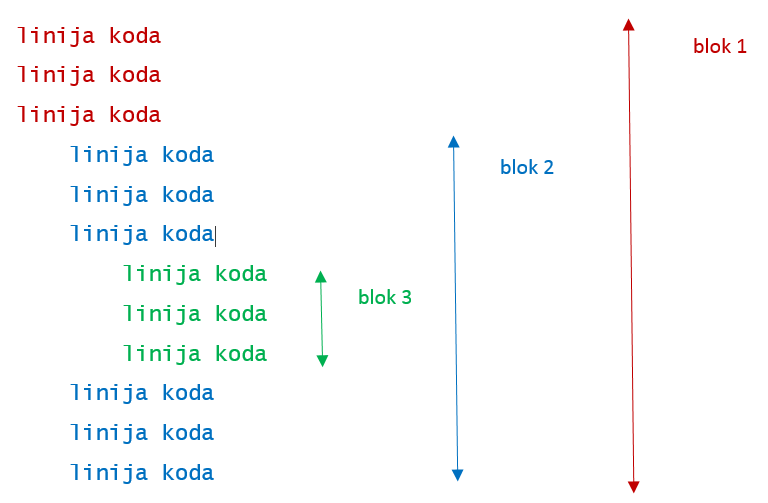
\includegraphics[scale=0.5]{whitespace.png}
\caption{Пример програмских блокова у Python-у}
\label{slike:whitespace}
\end{figure}

\subsubsection{Наредба if}

Следи начин на који би се претходно питање, тј. услов, могао реализовати:

\begin{lstlisting}[caption = Пример услова, label = if]
>>> godine_studiranja = 6
>>> if godine_studiranja < 8:
      print('Vi ste sjajan student')
\end{lstlisting}

\subsubsection{Наредба if-then-else}

Могуће је проширити дефиницију \emph{if} наредбе како би, на пример у претдном примеру пронашло колико је ко година студирао. За такву структуру је потребна кључна реч \emph{else}\index{Python!else@\emph{else}}.

Укратко, ако је услов у \emph{if} делу тачан, извршава се блок испод те линије, а ако није тачан, извршава се блок испод \emph{else} линије ако та линија кода постоји. Ако не постоји, а услов није тачан, неће се ништа извршити, већ интепретатор наставља извршавање даљих линија к\^{о}да.

\begin{lstlisting}[caption = Пример за наредбе IF - ELSE, label = ifelse]
>>> if godine_studiranja < 8:
        print('Vi ste sjajan student')
    else:
        print('Nije strasno')
\end{lstlisting}

\subsubsection{Услови и комбиновање услова}

Упоређивање две величине даје једну од две вредности: тачно или нетачно. Следећи оператори се користе за упоређивање:

\begin{table}[here]
\centering
\begin{tabular}{|c|c|} \hline
\textbf{Оператор} & \textbf{Дефиниција} \\ \hline \hline
== & једнако \\ \hline
!= & није једнако \\ \hline
> & веће од  \\ \hline
< & мање од \\ \hline
>= & није мање од \\ \hline
<= & није веће од \\ \hline
\end{tabular}\medskip
\caption{Оператори упоређивања}
\label{tabele:opporedjenja}
\end{table}

На пример, ако је потребно проверити да ли нека особа има 20 година, користи се оператор једнакости: \emph{if godine==20:}

Услови се комбинују коришћењем логичких оператора \emph{и} и \emph{или}. Оператор конјункције је \emph{and}, а дисјункције \emph{or}. Тако да на пример можемо овако рећи: \emph{if godine > 18 and bodovi >=50:} и слично.
